\documentclass{article}[twocolumn]
\usepackage[pdftex]{graphicx}
\usepackage[utf8]{inputenc}
\usepackage[brazil]{babel}
\usepackage{subfigure}
\usepackage{mathtools}
\usepackage{amsmath}
\usepackage{amssymb}
\usepackage{float}
\usepackage{tikz}

\title{Lab 1}
\author{Kenji Yamane}

\begin{document}
	\maketitle
	\section{Quest\~ao 1}
	\begin{figure}[H]
		\centering
		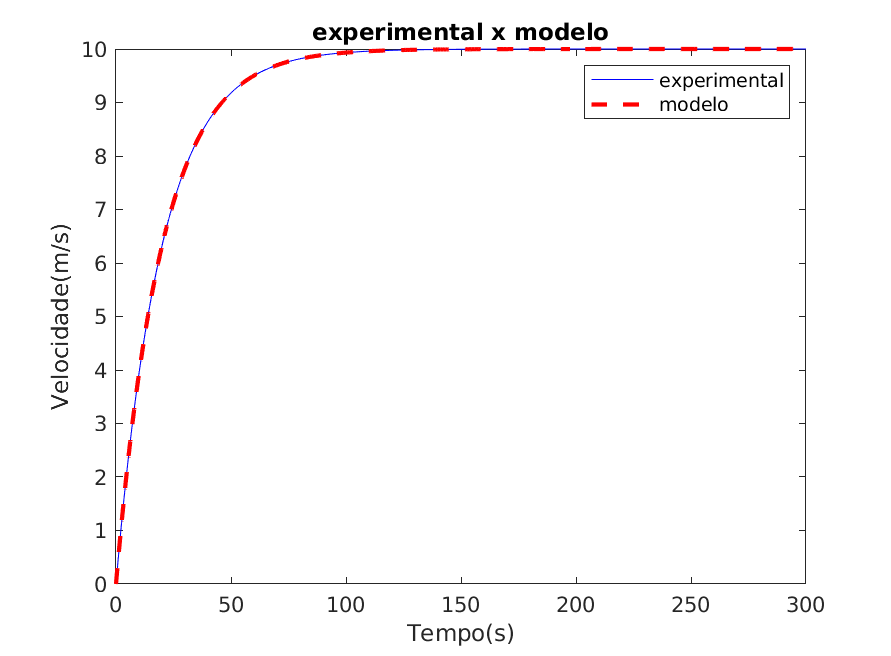
\includegraphics[width=7cm]{teste_modelo.png}
		\caption{Compara\c{c}\~ao entre o modelo e o experimento.}
	\end{figure}
	Pela figura obtida, percebe-se como s\~ao praticamente iguais as curvas obtidas,
	sendo dif\'icil de se notar alguma diferen\c{c}a a olho nu. Isso confirma como o modelo
	ao qual se chegou \'e coerente para o caso.
	\section{Quest\~ao 2}
	\subsection{a}
	\begin{figure}[H]
		\centering
		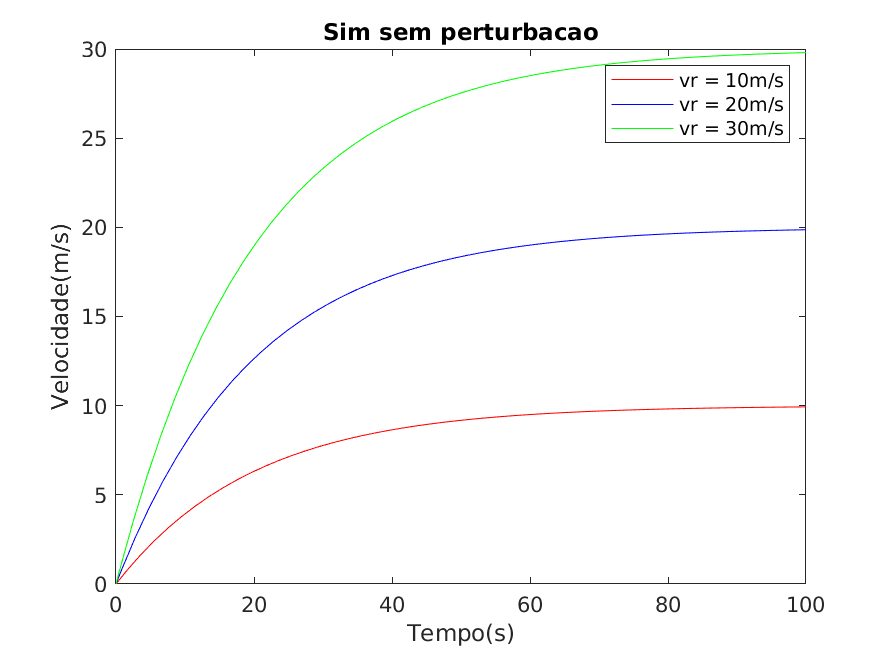
\includegraphics[width=7cm]{2a.png}
		\caption{Desempenho da malha aberta em casos nominais.}
	\end{figure}
	Verifica-se como a malha aberta \'e eficiente em atingir a velocidade requerida, em
	casos nominais, dado que eventualmente as tr\^es curvas se estabilizam no valor requerido.
	\subsection{b}
	\begin{figure}[H]
		\centering
		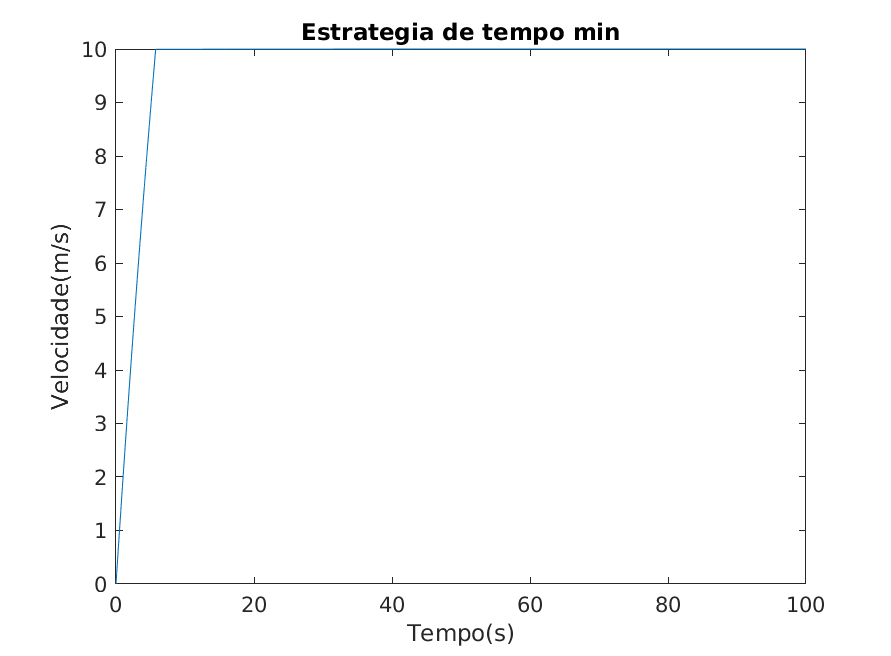
\includegraphics[width=7cm]{2b.png}
		\caption{Implementa\c{c}\~ao da estrat\'egia de tempo m\'inimo.}
	\end{figure}
	Observando a figura, nota-se como a malha aberta possui um desempenho impressionante
	quando se busca o tempo m\'inimo, se estabilizando em um valor de velocidade bem pr\'oximo
	do requerido. Todavia, deve-se lembrar que ainda est\'a se tratando de casos nominais.
	\subsection{c}
	\begin{figure}[H]
		\centering
		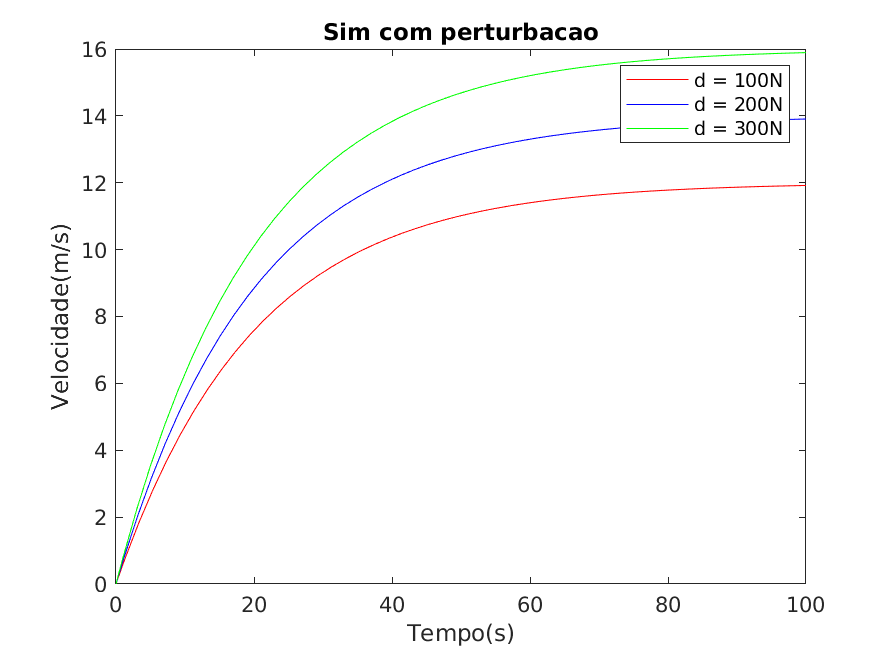
\includegraphics[width=7cm]{2c.png}
		\caption{Desempenho da malha aberta sob perturba\c{c}\~ao.}
	\end{figure}
	Como esperado, verifica-se que a malha aberta somente possui desempenhos favor\'aveis
	em situa\c{c}\~oes idealizadas. Verifica-se erro em regime, positivo, como previsto
	pela teoria.
	\subsection{d}
	\begin{figure}[H]
		\centering
		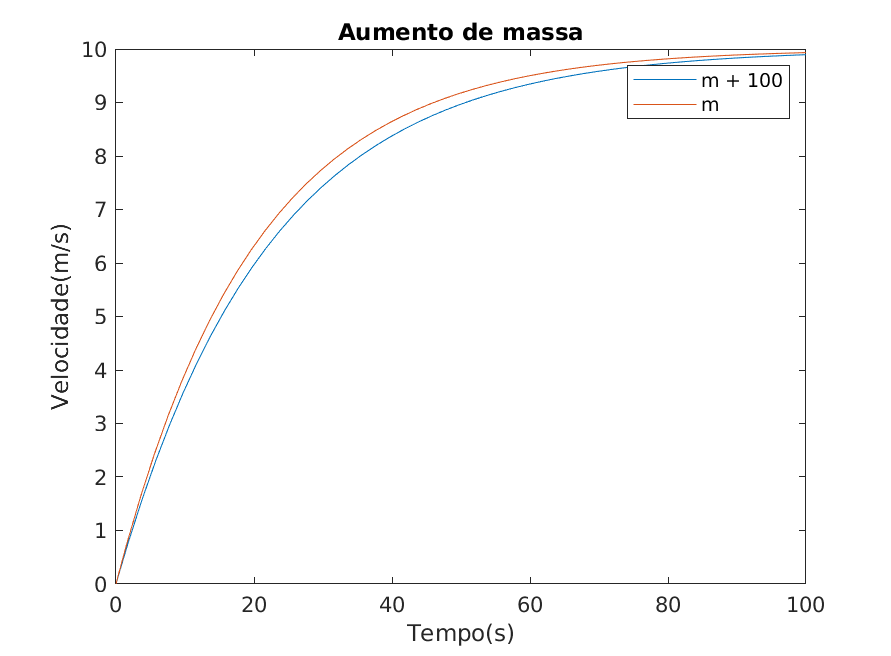
\includegraphics[width=7cm]{2d.png}
		\caption{Desempenho da malha aberta sob mudan\c{c}a da massa.}
	\end{figure}
	Verifica-se pouco efeito da mudan\c{c}a da massa no desempenho da malha aberta, somente
	na in\'ercia de mudan\c{c}a da curva. Isso era esperado, pois a massa n\~ao influencia na
	velocidade de regime, somente na constante de tempo. A diferen\c{c}a \'e pequena
	pois o erro foi de somente 3\%.
	\subsection{e}
	\begin{figure}[H]
		\centering
		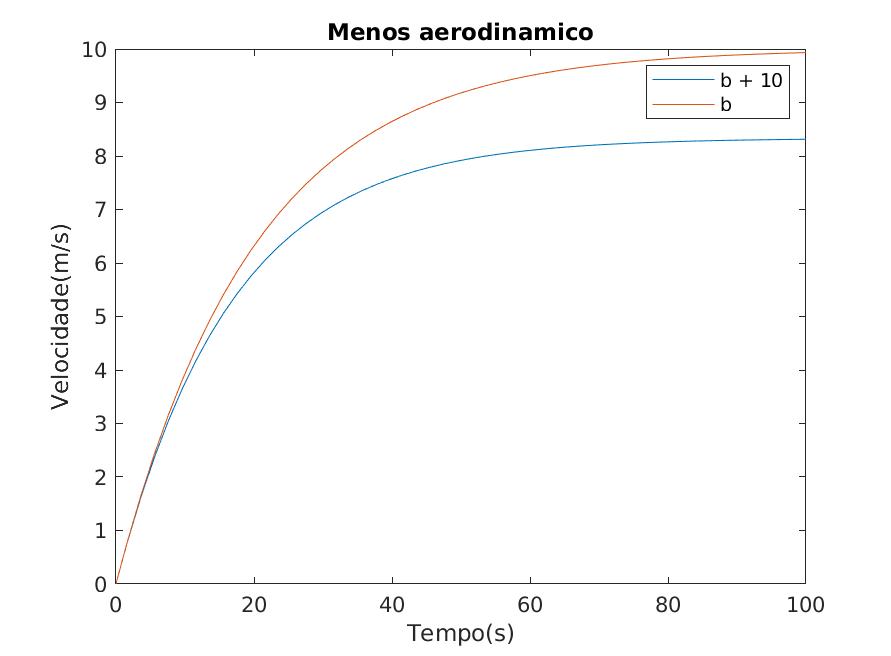
\includegraphics[width=7cm]{2e.png}
		\caption{Desempenho da malha aberta sob mudan\c{c}a do amortecimento.}
	\end{figure}
	Agora com rela\c{c}\~ao ao amortecimento, ele altera bastante a velocidade de regime, o
	que \'e natural dado que, quando projetado, o sistema de controle havia determinado u
	a partir de um b diferente do atual. Desta forma u est\'a diferente do necess\`ario
	para atingir a velocidade especificada.
	\section{Quest\~ao 3}
	\subsection{a}
	\begin{figure}[H]
		\centering
		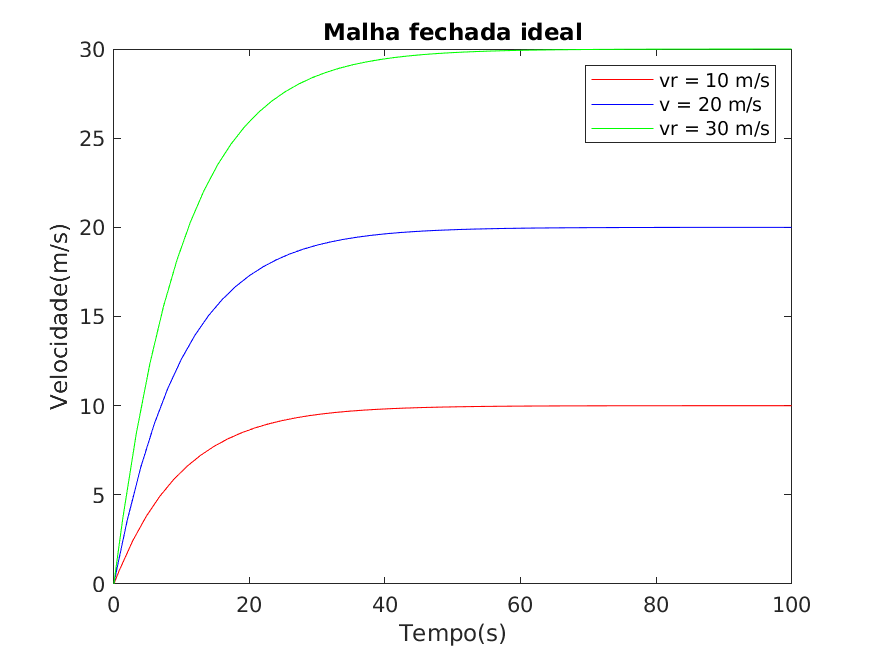
\includegraphics[width=7cm]{3a.png}
		\caption{Desempenho da malha fechada em caso nominal.}
	\end{figure}
	A malha fechada se demonstra correta nos casos nominais da mesma forma que na malha
	aberta. Isso decorre do fator \textit{feedforward} levado em conta, o qual recebeu o
	mesmo valor de b, o que anula o erro em regime.
	\subsection{b}
	\begin{figure}[H]
		\centering
		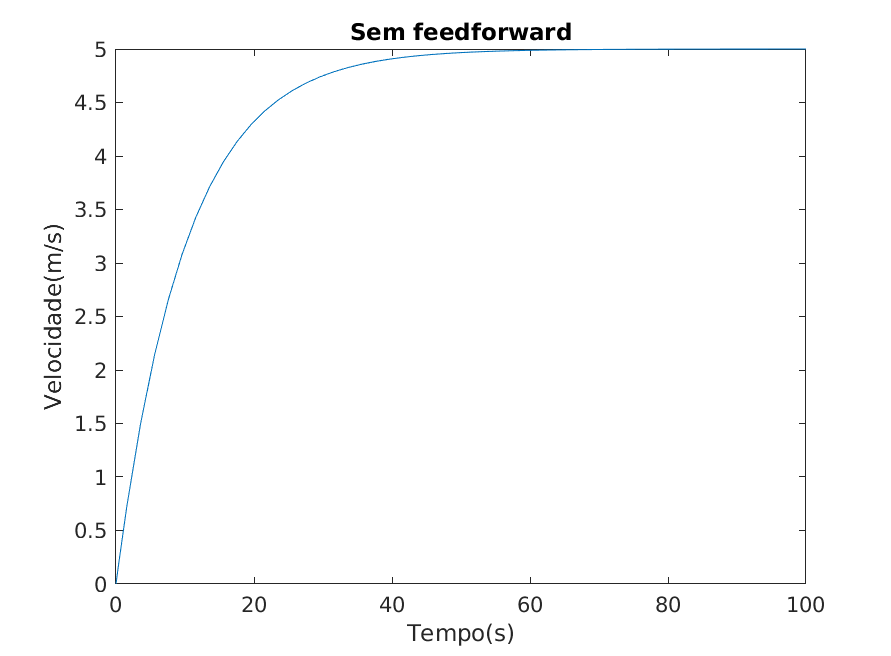
\includegraphics[width=7cm]{3b.png}
		\caption{Desempenho da malha fechada em caso nominal sem \textit{feedforward}.}
	\end{figure}
	A figura atual demonstra o que acontece se n\~ao \'e adicionado um fator
	\textit{feedforward}, a malha fechada erra bastante. O erro \'e condizente com a teoria,
	pois o valor de Kp \'e o mesmo da constante de amortecimento.
	\subsection{c}
	\begin{figure}[H]
		\centering
		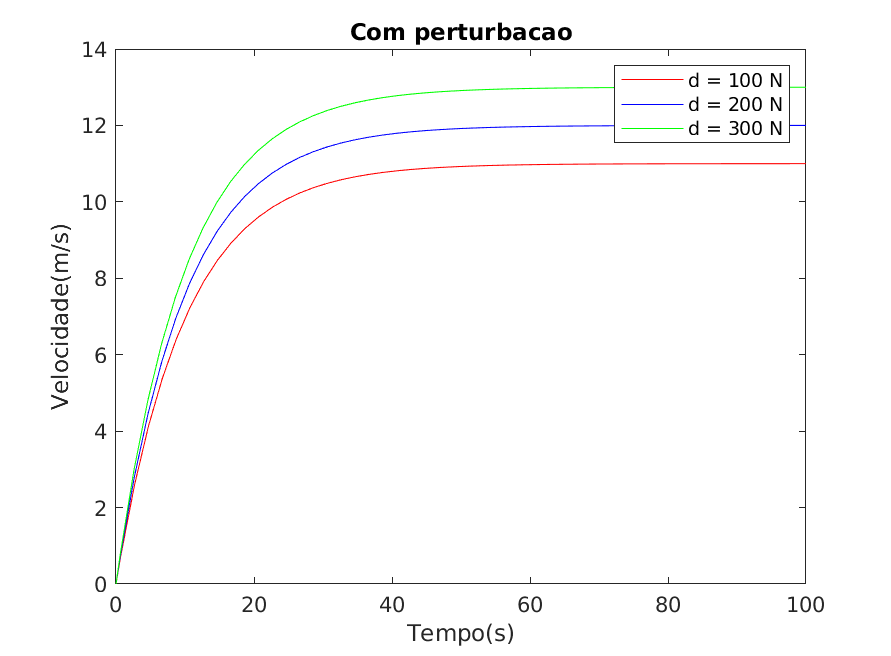
\includegraphics[width=7cm]{3c.png}
		\caption{Desempenho da malha fechada com perturba\c{c}\~ao.}
	\end{figure}
	Aqui, se confirma a robustez da malha fechada. O erro ainda ocorre, e \'e negativo, como
	esperado pela teoria e que nem na malha aberta. Por\'em, em compara\c{c}\~ao a este, o erro
	\'e bem menor. Ele poderia ser ainda menor, com um aumento do Kp.
	\subsection{d}
	\begin{figure}[H]
		\centering
		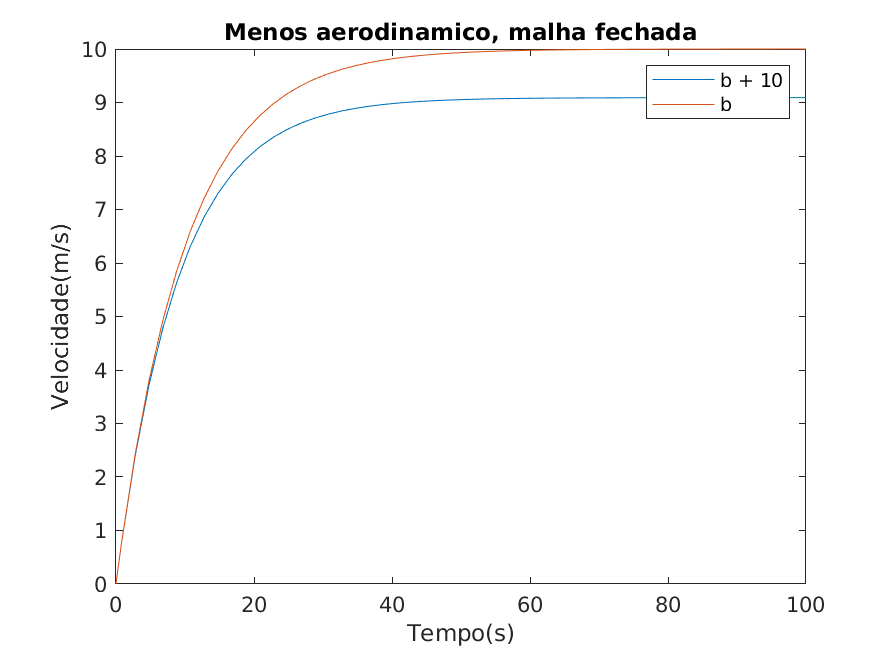
\includegraphics[width=7cm]{3d.png}
		\caption{Desempenho da malha fechada com mudan\c{c}a do amortecimento.}
	\end{figure}
	Novamente outro refor\c{c}o da robustez da malha fechada em rela\c{c}\~ao a aberta,
	o erro em virtude da mudan\c{c}a do amortecimento \'e bem menor. Dessa vez o erro
	ocorre de fato pois o amortecimento influencia na velocidade de refer\^encia.
	\subsection{e}
	\begin{figure}[H]
		\centering
		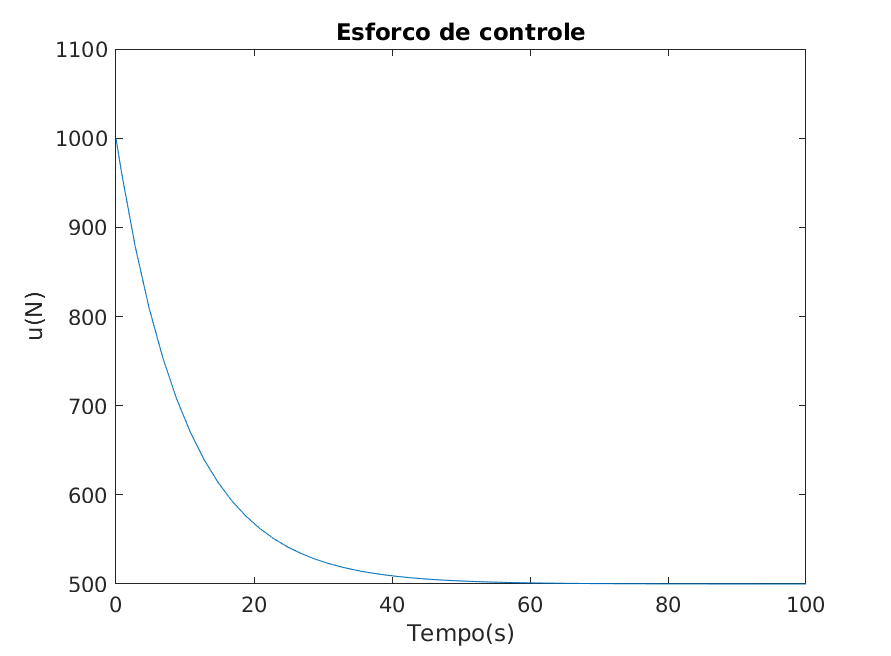
\includegraphics[width=7cm]{3e.png}
		\caption{Esfor\c{c}o do controle para o caso nominal.}
	\end{figure}
	Aqui se observa a for\c{c}a necess\'aria em cada instante para que o controle em malha
	fechada ocorra. \'E relativamente alta. Se comparada com a estrat\'egia de tempo
	m\'inimo da malha aberta, \'e bem menor, \`as custas entretanto de um tempo bem maior
	para se atingir o regime. Todavia isso tudo \'e regul\'avel na malha fechada, o que mostra
	a maior maleabilidade e robustez da malha fechada.
\end{document}
